\documentclass[12pt, letterpaper]{article}
\title{Phaktionz TCG Official Rules Handbook}
\author{Casual Card Cafe | Phaktionz Rules Commitee}
\date{Version 1.3}
\usepackage{color}
\usepackage{hyperref}
\usepackage{graphicx}
\usepackage{caption}
\hypersetup{
colorlinks=true, % make the links colored
linkcolor=black, % color TOC links in blue
urlcolor=red, % color URLs in red
linktoc=all % 'all' will create links for everything in the TOC
}
%\usepackage{times}
\begin{document}
\maketitle
\pagenumbering{arabic}
\newpage
\tableofcontents
\newpage
\begin{center}
    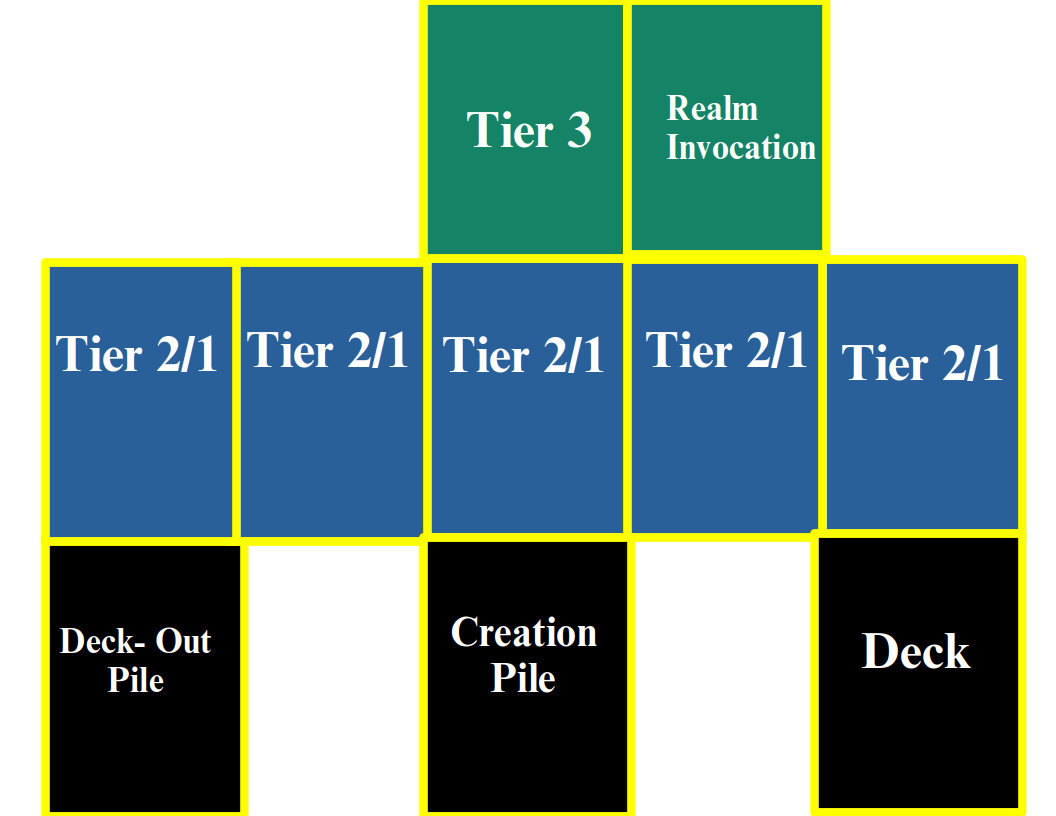
\includegraphics[scale = 0.25]{images/field.png}
    \captionof{figure}{Battlefiled Layout Version 1}
\end{center}


\section{Rules}
\paragraph{How to Win\\}
To win you must deck out your opponent, or in other words bring their deck to 0 cards, where no more cards can be drawn.
\subsection{Formats}
In any format: 
\begin{itemize}
    \item A player can only have 4 copies of a single card unless specified any exception
    \item A player must start with 5 cards in their hand 
    \item A player's turn has the following phases:
     \begin{itemize}
        \item Draw Phase (Player draws a card from their deck)
        \item Main Phase (Can place summons or cast invocations)
        \item Combat Phase (Battle using your summons)
        \item Final Cast (Can only cast invocations)
        \item End Phase (Ends turn)
     \end{itemize}
\end{itemize}
\paragraph{Standard (Version 1.1.3): \\}
\begin{itemize}
    \item This format is the most common format that is played, and considered the default playing style. 
    \item A Deck must contain 50 cards 
    \item A Deck must contain Summons belonging to only one Faction. 
\end{itemize}
\paragraph{Synthesis (Version 2.1.3): \\}
\begin{itemize}
    \item This format is the mix and match sort of playstyle that will bring an interesting battle upon yourself. 
    \item A Deck must contain at least 50 cards, and a max of 75. 
    \item A Deck may contain Summons belonging to one or more Factions. 
        \begin{itemize}
            \item Must contain Summons from each Faction in each Tier being played
        \end{itemize}
    \item Origins may be used in a combination of Unknowns and Modernas Factions. 
    \item Unknowns and Modernas Factions may not be combined together. 
\end{itemize}
\newpage
\subsection{Types of Cards}
\paragraph{Summons: \\}
\par These are your soldiers that battle on the battlefield against your opponent. 
\par A Summon has the following information: 
\begin{itemize}
    \item Tier: A Summon can have a Tier from 0 - 4
    \item Type: There are two types of Summons 
    \begin{itemize}
        \item Strikers:  can battle any opponent's Summons but not directly
        \item Tech: can only battle opposing summons in the same column, but if there are no opposing summons in their column they can battle directly.
    \end{itemize}
    \item DMG: The amount of Damage a Summon can deal to an Opponent
    \item Faction: The Faction in which the Summon belongs to (ex. Mythicals or Probers)
\end{itemize}
\paragraph{Invocations: \\}
\par These are a type of magic or sorcery that may be cast on the battlefield 
\par An invocation has the following information: 
\begin{itemize}
    \item Type: 
    \begin{itemize}
        \item Regular: This type of invocation may only be cast on your turn 
        \item Counter: This type of invocation may be cast on any turn
        \item Realm: This type of invocation remains on the battlefield
        \item Weapon: This type of invocation attaches itself to a Summon on the battlefield
    \end{itemize}
\end{itemize}
\newpage
\subsection{Terms}
\paragraph{Keywords: }
\begin{itemize}
    \item Summons: Units that battle in the battlefield
    \item Invocations: Sorcery that may be cast to gain benefit. 
    \item Abled: The position in which a unit may battle 
    \item Disabled: The position in which a unit is unable to battle (This is done with your Summon being sideways)
    \item Demote: To have a summon leave the battlefield
    \item Exile: To remove from play a summon
    \item Tiers: Represents the rank of a summon, Tier 1 being the lowest and 3 the highest
    \item DMG: The amount of cards a summon can deal an opponent to lose, this is indicated on the card, and when battles an opposing summon, is dealt the difference.
    \item Fizzle: To stop an opponent's play 
\end{itemize}
\paragraph{Conditions:}
\begin{itemize}
    \item L/x: Limit x per turn
    \item Lx: Limit x per match
\end{itemize}
\newpage
\subsection{Game Mechanics}
\paragraph{Game Mechanics: \\}
\begin{itemize}
    \item When a Summon battles it becomes disabled (turned sideways)
    \item To place a Tier 2 or higher summon, you must demote Tiers total to the Summon's Tier. 
    For example, a Tier 2 may be placed by demoting a Tier 2 or 2 Tier 1s.
    \item At the start of the game, after the turn order is chosen, both players may mulligan any cards in their hand once.
    \item If a card’s ability were to break one of these rules, the card's ability takes precedence.
    \item When battling, a Player takes DMG equal to the difference between the Summons. 
    \begin{itemize}
        \item If a Summon that battles has less DMG than the opposing, no DMG is dealt.
        \item If a Summon that battles has more DMG than the opposing, the Opponent takes the difference, 
        and the Summon is demoted, except if it's Tier 3+. 
    \end{itemize} 
\end{itemize}

\newpage
\subsection{Creation Pile}
Creation Pile is a pile located in the middle between your Deck and Deck Out Pile. It's basic function is that 
cards in it may be added to your hand if they satisfy the Card's Create condition. 

\begin{itemize}
    \item Limit: 10 (In Format V1 \& V2)
    \item Abilities that include 'CP' refer to Creation Pile
    \item The goal of Creation Pile is have a last resort to yourself
    \item CP Cards are identified with CP in the top left along where Tier or Invocation type is located. 
\end{itemize}
\end{document}